\section{Work Plan}

Our work plan consists of a work breakdown structure (Figure \ref{fig:workplan}) and a Gantt chart (Figure \ref{fig:gantt-chart}).
We identified 5 principal components, each successive component has a dependency on, and cannot start before, the previous component being completed, which represents a milestone.

% Generated by https://online.visual-paradigm.com/
\begin{figure}[h]
\centering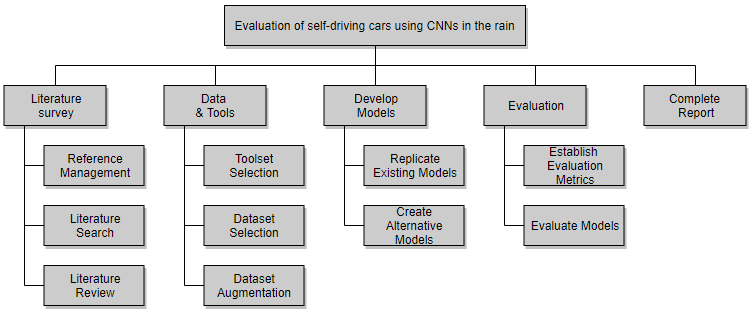
\includegraphics[width=1\linewidth]{figures/work-breakdown-structure.png}
\caption{Work breakdown structure}
\label{fig:workplan}
\end{figure}

\begin{figure}[h]
\begin{center}
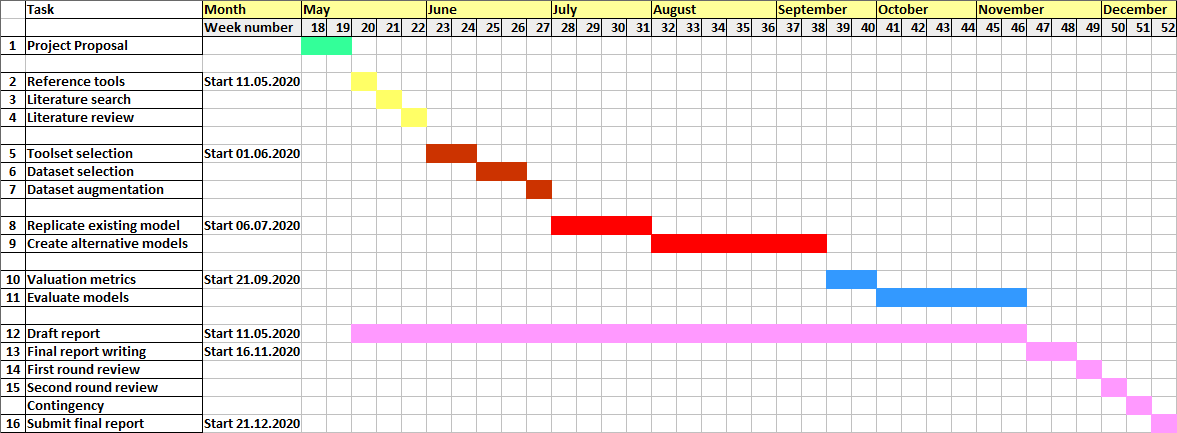
\includegraphics[scale=0.55] {figures/gantt-chart-v3.png}
\caption{Gantt chart}
\label{fig:gantt-chart}
\end{center}
\end{figure}




